\chapter{Integrals and ratios}
\label{ch:spectral_preprocessing}


\begin{wrapfigure}{o}{0.72\textwidth}
    \centering
    \vspace{-3cm}
    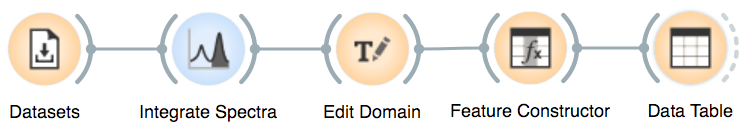
\includegraphics[width=0.85\textwidth]{integrals-ratios-fig1.png}
    \label{fig:integrals-ratios-fig1}
\end{wrapfigure}

Peak integration is an essential element of spectroscopy for measuring concentrations, spectral contributions, etc. 

\begin{wrapfigure}{o}{0.95\textwidth}
    \centering
    % \vspace{-1cm}
    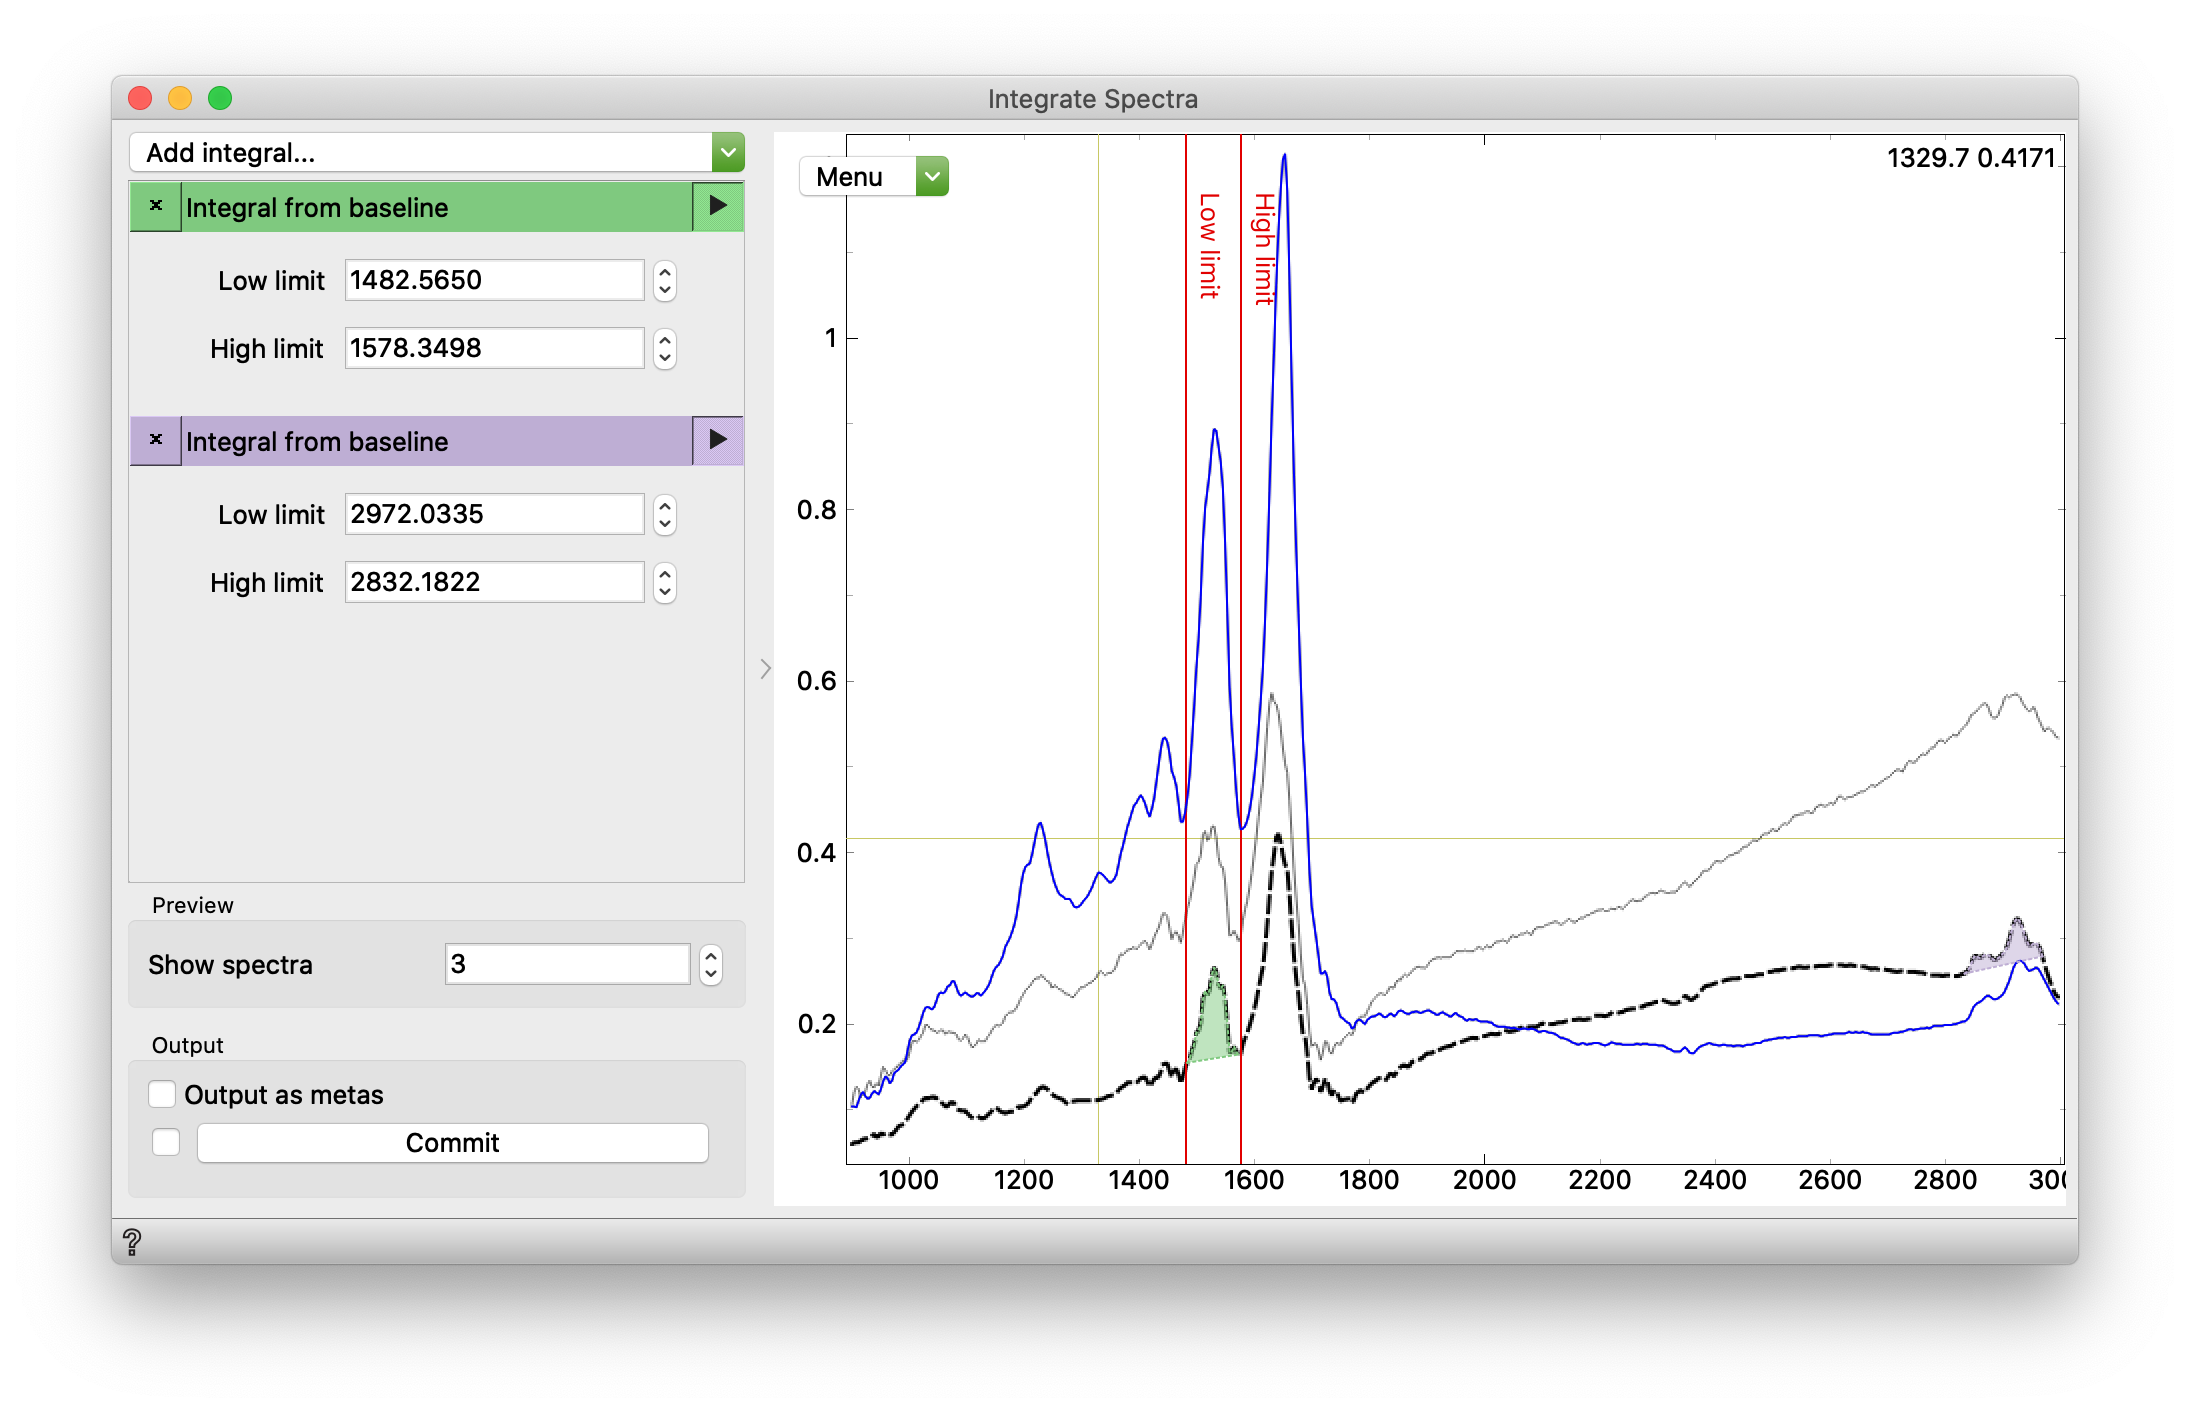
\includegraphics[width=\textwidth]{integrals-ratios-fig2.png}
    \caption{To display a preview, select a spectrum and enable preview of individual integrals with their play buttons.}
    \label{fig:integrals-ratios-fig2}
\end{wrapfigure}

To compute integrals, we use the \textit{Integrate Spectra} widget. Let’s compute the ratios of two integrals to establish an internal standard in our dataset. Add two integrals and then feed them into the \textit{Feature Constructor} (\textit{Edit Domain} is optional—we use it to simplify column names). In \textit{Feature Constructor}, we can create new numeric features with Python expressions.
To work with Feature Constructor more easily, uncheck “Output as metas”, which will replace the original spectra with their integrals (and reduce the number of columns in your data).
We can use \textit{Feature Constructor} whenever we would like to create a new column from existing data. 

\begin{figure}[h]
\vspace{-0.5cm}

\stackinset{r}{-0.65\linewidth}{t}{+0.15\linewidth}
% {r} is left-right
% {t} is top-bottom
  {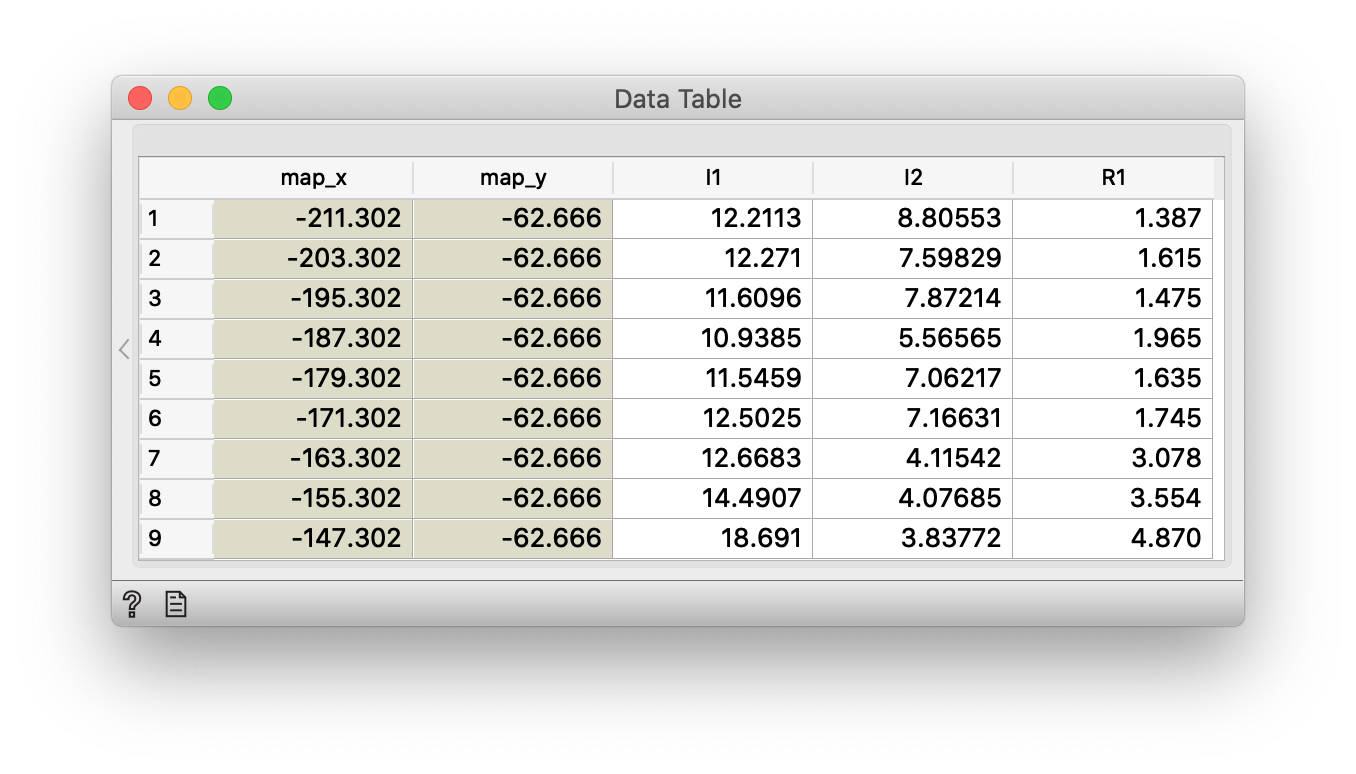
\includegraphics[scale=0.45]{integrals-ratios-fig4.png}}
  {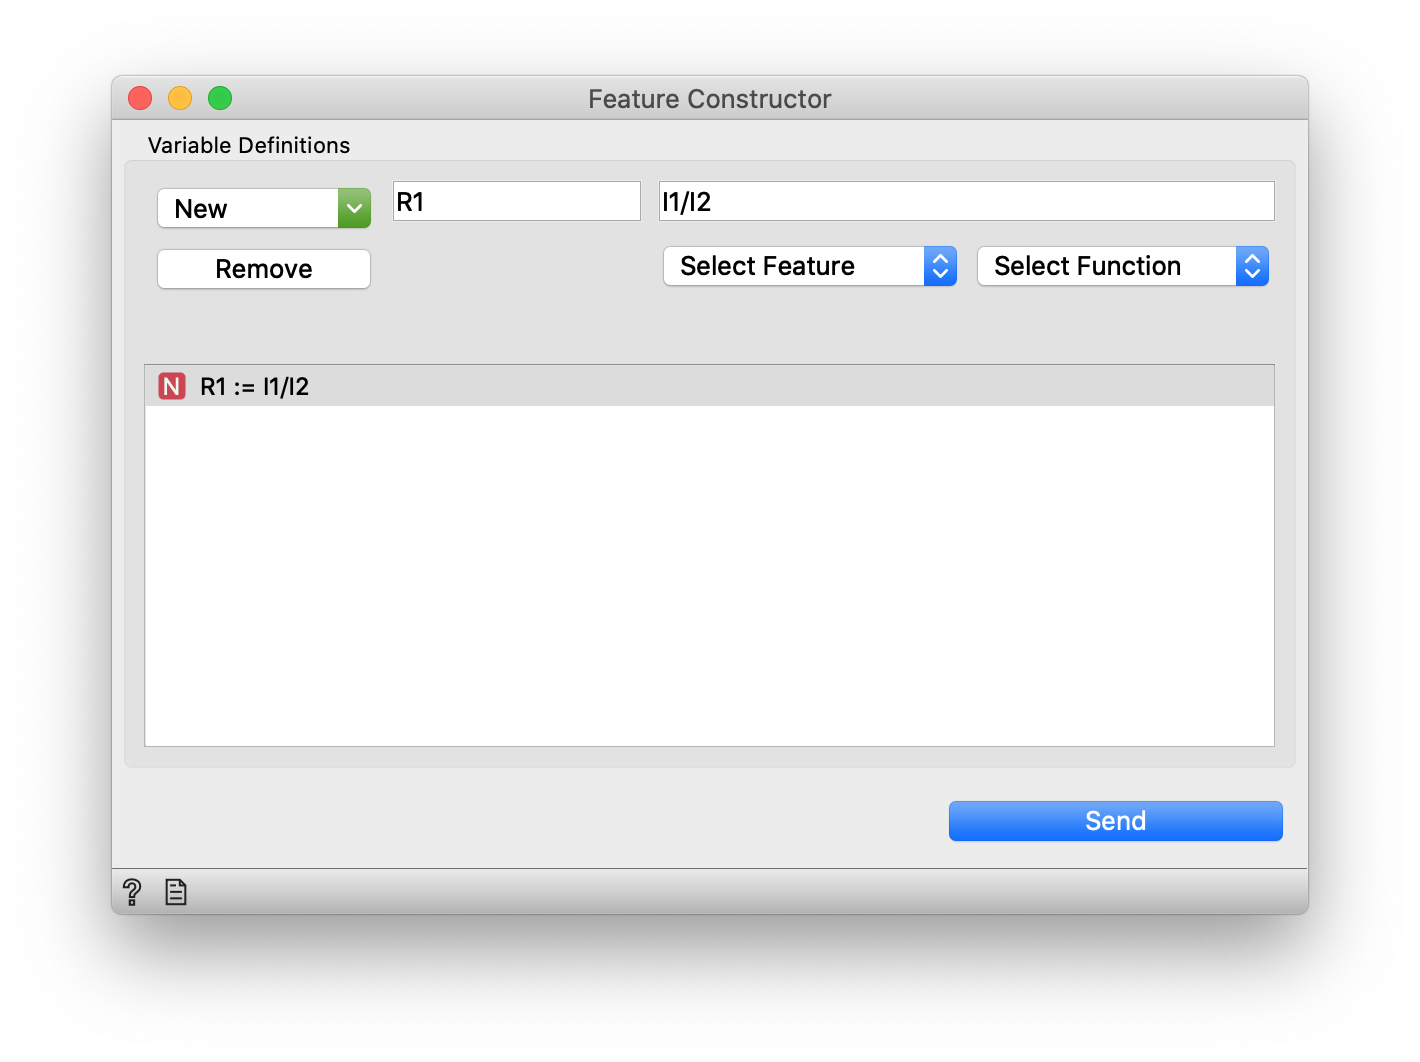
\includegraphics[scale=0.4]{integrals-ratios-fig3.png}}
  \caption{We added a Numeric feature, the ratio of I1 and I2 called R1.}
  \label{fig:spectral-PCA-fig2}
\end{figure}

\noindent The produced data can be inspected by connecting other widgets.